\scanpage{131}
% E01: printed listing.
{\ttfamily\small
\$HASP373 STARTED - INIT 1 - CLASS 1 - SYS E333\par
IEF236I ALLOC. FOR CRAY2\par
IEF142I CRAY2 - STEP WAS EXECUTED - COND CODE 0000\par
IEF373I STEP /\qquad / START 82228.1615\par
IEF374I STEP /\qquad / STOP 82228.1615 CPU 0MIN 00.02SEC SRB\quad 0MIN 00.00SEC VIRT\qquad 8K SYS\quad 164K\par
IEF375I JOB /CRAY2\quad / START 82228.1615\par
IEF376I JOB /CRAY2\quad / STOP 82228.1615 CPU\quad 0MIN 00.02SEC SRB\quad 0MIN 00.00SEC\par}

\figure{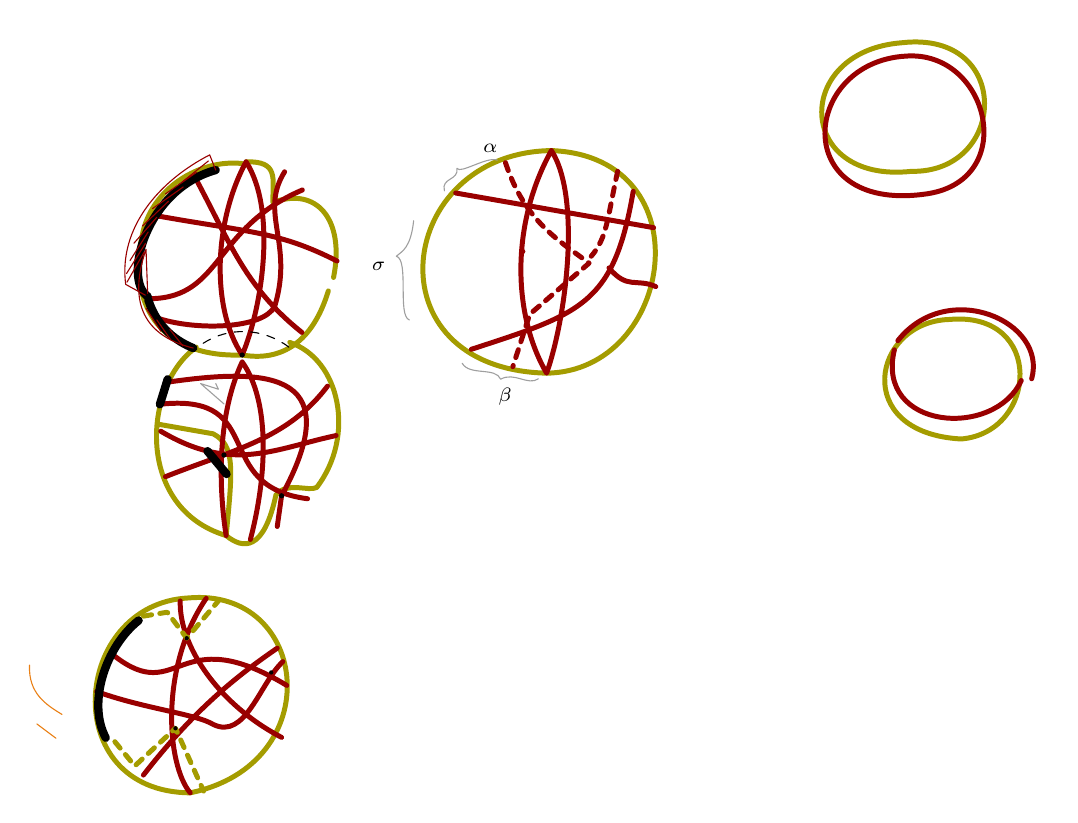
\begin{tikzpicture}[x=.55cm,y=-.55cm,line cap=round,line join=round,g/.style={olive!80!yellow,line width=1.8pt},r/.style={red!60!black,line width=1.8pt},p/.style={gray!75,thin},every node/.style={font=\scriptsize}]
% E02: joined arrangements at left, marked and overtraced boundary.
\draw[g] (7.88,5.32)..controls(8.65,5.3)and(8.49,5.71)..(8.5,6.26)..controls(9.5,5.88)and(10.17,6.64)..(9.9,7.99) (9.78,8.3)..controls(9.42,9.48)and(8.71,9.94)..(7.79,9.78)..controls(5.82,9.85)and(5.15,8.51)..(5.48,7.03)..controls(5.68,5.93)and(6.82,5.25)..(7.79,5.36);
\draw[g] (6.73,9.6)..controls(5.49,10.48)and(5.31,13.32)..(7.42,13.95)..controls(7.57,12.4)and(7.63,11.87)..(7.12,11.6)--(5.86,11.38) (7.42,13.95)..controls(7.81,14.27)and(8.29,14.32)..(8.57,13.01)..controls(8.84,12.69)and(9.31,12.94)..(9.51,12.84)..controls(10.42,11.65)and(10.05,9.88)..(8.89,9.49);
\draw[r] (7.88,5.32)..controls(8.6,6.44)and(8.25,8.7)..(7.79,9.78)..controls(7.07,8.7)and(7.13,6.71)..(7.88,5.32) (6.73,5.73)..controls(7.53,7.23)and(7.87,8.22)..(9.17,9.26) (5.84,6.57)..controls(7.97,6.95)and(8.64,6.93)..(9.98,7.61) (5.68,8.48)..controls(7.33,8.45)and(7.12,6.85)..(9.18,5.97) (5.87,8.94)..controls(6.75,9.22)and(8.27,9.18)..(8.54,8.66)..controls(8.99,7.19)and(8.17,6.51)..(8.77,5.55);
\draw[r] (7.79,9.94)..controls(8.45,10.87)and(8.36,12.59)..(7.98,14.04) (7.79,9.94)..controls(7.23,11.14)and(7.23,12.73)..(7.42,13.95) (6.05,10.41)..controls(8.15,10.11)and(10.34,10.03)..(8.7,13.03)--(8.6,13.74) (5.97,10.91)..controls(8.38,10.69)and(7.05,12.81)..(9.3,13.1) (5.91,11.54)..controls(7.56,12.52)and(8.55,11.94)..(9.96,11.64) (6.02,12.59)..controls(7.58,11.97)and(8.83,11.73)..(9.76,10.5);
\draw[line width=3pt] (7.18,5.51)..controls(5.55,5.96)and(5.03,8.03)..(5.61,8.43) (5.62,8.5)..controls(5.83,9.17)and(6.31,9.48)..(6.66,9.62) (6.07,10.34)--(5.89,10.92) (6.99,12.0)--(7.43,12.53);
\draw[r,thin] (7.18,5.51)--(7.04,5.16)..controls(5.89,5.75)and(4.93,6.83)..(5.1,8.15)--(5.61,8.43)--(5.57,7.34)..controls(5.09,8.74)and(5.69,9.38)..(6.66,9.62);
\foreach \x/\y/\u/\v in {5.13/8.1/5.53/7.4,5.12/7.9/5.56/7.2,5.2/7.6/5.62/6.94,5.29/7.2/5.82/6.6,5.49/6.8/6.09/6.23,5.72/6.4/6.43/5.9,6.02/6.06/6.74/5.56,6.4/5.79/7.01/5.3,5.57/8.7/5.91/9.23,5.82/8.97/6.14/9.43,6.12/9.19/6.42/9.57}{\draw[r,thin] (\x,\y)--(\u,\v);}
\draw[dashed] (6.89,9.51)..controls(7.47,9.13)and(8.26,9.14)..(8.87,9.6);
\foreach \x/\y in {5.61/8.43,7.79/9.78,7.37/12.09,8.7/13.03}{\fill (\x,\y) circle (.06);}
\draw[p] (6.83,10.44)--(7.37,10.91) (6.83,10.44)--(7.24,10.57)--(7.18,10.44);
% E03: central arrangement and three pencil braces with labels.
\draw[g] (14.93,5.06)..controls(18.5,5.2)and(17.77,10.16)..(14.82,10.2)..controls(10.68,10.1)and(11.32,5.11)..(14.93,5.06);
\draw[r] (14.93,5.06)..controls(15.62,6.13)and(15.28,8.89)..(14.82,10.2)..controls(14.03,8.84)and(13.99,6.75)..(14.93,5.06) (12.72,6.04)--(17.29,6.84) (13.08,9.65)..controls(15.62,8.82)and(16.37,8.62)..(16.82,6.0);
\draw[r,dashed] (13.87,5.34)..controls(14.32,6.71)and(15.13,7.15)..(15.8,7.66)--(14.43,8.84)--(14.04,10.05) (16.46,5.54)..controls(16.22,6.63)and(16.22,7.07)..(15.85,7.5);
\draw[r] (16.26,7.77)..controls(16.69,8.28)and(16.88,8.0)..(17.34,8.2);
\fill[red!60!black] (14.27,7.39) circle (.06); \fill[red!60!black] (15.19,8.17) circle (.045);
\draw[p] (13.68,5.28)..controls(13.44,5.19)and(12.82,5.61)..(12.75,5.47)..controls(12.79,5.76)and(12.38,5.68)..(12.46,5.99) (11.75,6.68)..controls(11.68,7.31)and(11.49,7.38)..(11.35,7.5)..controls(11.65,7.58)and(11.37,8.88)..(11.65,8.97) (12.87,9.97)..controls(13.04,10.27)and(13.64,10.05)..(13.76,10.34)..controls(14.07,10.16)and(14.39,10.5)..(14.63,10.33);
\node at (13.52,5.01) {$\alpha$}; \node at (10.94,7.73) {$\unsure{\sigma}$}; \node at (13.86,10.74) {$\beta$};
% E04 and E05: the two pairs of outlines at right.
\draw[g] (23.03,2.57)..controls(25.59,2.28)and(25.47,5.58)..(23.24,5.54)..controls(20.56,5.83)and(20.48,2.76)..(23.03,2.57);
\draw[r] (23.1,2.88)..controls(25.05,2.72)and(25.78,5.81)..(23.52,6.07)..controls(20.41,6.47)and(20.71,3.03)..(23.1,2.88);
\draw[g] (24.12,8.96)..controls(26.33,8.76)and(26.17,11.57)..(24.39,11.72)..controls(21.83,11.58)and(22.34,9.01)..(24.12,8.96);
\draw[r] (22.93,9.45)..controls(24.07,8.0)and(26.39,9.0)..(26.02,10.33) (25.78,10.37)..controls(25.17,11.72)and(22.4,11.52)..(22.85,9.66);
% E06: lower-left circle, red curves, highlighted boundary and dashed arcs.
\draw[g] (6.55,15.39)..controls(9.36,15.14)and(9.8,19.23)..(6.59,19.89)..controls(3.5,19.87)and(3.85,15.53)..(6.55,15.39);
\draw[r] (6.36,15.46)..controls(6.33,16.47)and(7.21,17.83)..(8.7,18.61) (6.96,15.4)..controls(5.88,16.98)and(6.04,19.23)..(6.59,19.89) (4.84,16.73)..controls(6.35,17.9)and(6.27,15.87)..(8.82,17.41) (4.43,17.55)..controls(5.49,17.94)and(6.73,18.07)..(7.12,18.31)..controls(7.87,18.68)and(8.2,17.35)..(8.73,16.86) (5.51,19.48)..controls(6.69,17.96)and(7.67,17.19)..(8.6,16.55);
\draw[line width=3pt] (5.4,15.91)..controls(4.63,16.52)and(4.21,17.82)..(4.64,18.62);
\draw[g,dashed] (5.51,15.81)--(6.06,15.72)--(6.51,16.32)--(7.24,15.46) (4.85,18.71)--(5.31,19.27)--(6.25,18.4)--(6.9,19.85);
\foreach \x/\y in {6.51/16.32,6.25/18.4,8.46/17.11}{\fill (\x,\y) circle (.05);}
\draw[orange!65!brown,thin] (2.88,16.94)..controls(2.85,17.6)and(3.27,17.86)..(3.63,18.08) (3.05,18.3)--(3.49,18.63);
\end{tikzpicture}}

% E07: pencil text and calculations to the right of the central figure.
\[\alpha+\unsure{\sigma}+1\quad\text{\unsure{intervalles}}\]
\[\frac{\alpha+\unsure{\sigma}+1}{2}\]
\[\frac{\beta+\unsure{\sigma}+1}{2}\]
% E08.
\[\frac{\alpha+\beta+2\unsure{\sigma}+2}{2}\leq\alpha+\beta+\unsure{\sigma}+1\quad\unsure{\ast}\unsure{?|!}\]
% E09: cancelled working, including the final incomplete relation.
\[\deleted{\unsure{\alpha+\beta+\sigma+1}\quad\unsure{3}\,\frac{\alpha+\beta}{2}\,\unsure{\leq}}\]
% E10.
\[\frac{\alpha\unsure{+|-}\beta}{2}\quad\text{est \unsure{la différence}}\quad(\unsure{\geq}1\]
\margin{\mspage{130}}
